\documentclass[11pt,a4paper]{article}
\usepackage[dvipsnames]{xcolor}
\usepackage[utf8]{inputenc}
\usepackage{amsmath}
\usepackage{mathtools}
\usepackage{marvosym}
\usepackage{wrapfig}
\usepackage{hyperref}
\usepackage{float}
\usepackage{multicol}
\hypersetup{colorlinks,citecolor=black,filecolor=black,linkcolor=black,urlcolor=black}
\usepackage{pdfpages}
\usepackage{amsfonts}
\usepackage{amssymb}
\usepackage{fancyhdr}
\usepackage{chemfig}
\usepackage{graphicx}
\usepackage{t1enc}
\usepackage[magyar]{babel}
\usepackage{bm}
\usepackage{tikz, tcolorbox}
\usepackage{verbatim}
\usepackage{amsmath,esint}
\usepackage{setspace}
\usepackage{qtree}
\usepackage{multido}
\newcommand{\Pointilles}[1]{%
\par\nobreak
\noindent\rule{0pt}{1.5\baselineskip}% Provides a larger gap between the preceding paragraph and the dots
\multido{}{#1}{\noindent\makebox[\linewidth]{\dotfill}\endgraf}
\bigskip% Gap between dots and next paragraph
}
\usepackage{pgfplots}
\pgfplotsset{height = 10cm, width=15cm,compat=1.5}
\usepackage[left=2cm,right=2cm,top=2cm,bottom=2cm]{geometry}
\setlength{\parindent}{0pt}
\setlength{\parskip}{0em}
%\pagestyle{fancy}
\fancyhf{}
\cfoot{\thepage. oldal}
\begin{document}

\begin{titlepage}
\centering

\includegraphics[width=.8\textwidth]{bme_logo_nagy.jpg}

\vspace{1em}

{
\Large
BUDAPESTI MŰSZAKI ÉS GAZDASÁGTUDOMÁNYI EGYETEM GÉPÉSZMÉRNÖKI KAR
}

\vspace{10em}

{
\Huge
\textbf{Dinamika 1 Zh. feladatok}
}

\vspace{5em}

{
\huge
Tárgynév

\vspace{.2em}

\large
(BMEGEMMBXM3)
}

\vspace{4em}

{
\Large
\textit{Készítette:}\\
\vspace{.5em}
\textbf{Kis Erhard, Kun László Ákos}
}

\vspace{20em}

{
\large
BUDAPEST, 2023
}
\end{titlepage}
%------------------------------------------------------------------------------------------
%------------------------------------------------------------------------------------------
%------------------------------------------------------------------------------------------
\newpage
\setstretch{1.5}
\begin{center}
    \textbf{\LARGE{Dinamika}}\\
    1. Zárthelyi\\
    2009.10.13. A csoport
\end{center}
Az ábrán vázolt mechanizmus egy rögzített csúszkából és három rúdból áll. A rudak egymáshoz
csuklósan kapcsolódnak. A (2) és (3) jelű rudak egymással pillanatnyilag derékszöget zárnak be.
Ismert az (1) rúd \textbf{A} végpontjának pillanatnyi sebessége és a (2) rúd pillanatnyi szöggyorsulása.\\\\
\textbf{Adatok:}\\
\begin{tabular}{| c | c |}
    \hline
    $l_2$ & $0,1 [m]$\\ 
    \hline
    $l_3$ &  $0,2 [m]$\\  
    \hline
    $\varphi$ & $45 [^\circ]$\\  
    \hline
    $\varepsilon_2$ & $10 \left[\frac{rad}{s^2}\right]$\\
    \hline
\end{tabular}
\begin{center}
    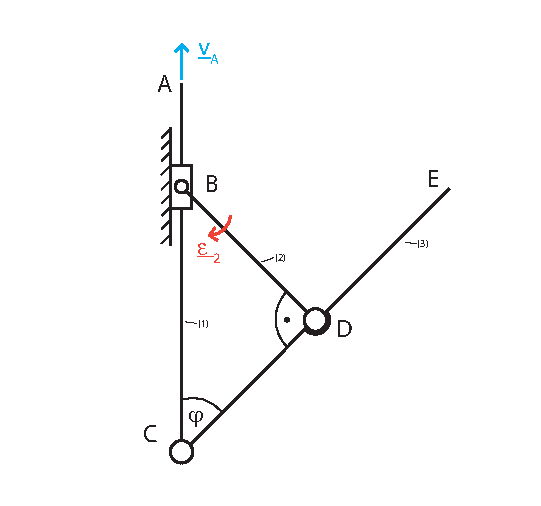
\includegraphics[width=.45\paperwidth]{Képek/2009.10.13_A.pdf}
\end{center}

\vspace{2em}
\underline{\textbf{Feladatok:}}
\begin{enumerate}
    \item Rajzolja be az ábrába a (3) rúd pillanatnyi sebességpólusát! Határozza meg az E pont
    sebességét!
    \item Adja meg a (3) rúd szöggyorsulását és számitsa ki az A pont pillanatnyi
    \item Készítsen külön ábrát és jelleghelyesen adja meg a (3) rúd gyorsuláspólusának helyét!
    \item Vizsgálja az (1) rúd C pontjának mozgását a (2) rúdhoz képest! Készitsen külön ábrát és
    jelleghelyesen rajzolja be a C pont szállitó-és relativ sebességét, valamint a C pont
    Coriolis gyorsulását!
\end{enumerate}

%------------------------------------------------------------------------------------------
%------------------------------------------------------------------------------------------
%------------------------------------------------------------------------------------------

\newpage

\setstretch{1.5}
\begin{center}
    \textbf{\LARGE{Dinamika}}\\
    1. Zárthelyi\\
    2009.10.13. B csoport
\end{center}
Az ábrán vazolt mechanizmus egy rögzitett csúszkából és három rúdból áll. A rudak egymáshoz
esuklósan kapcsolódnak. A (1) és (2) jelü rudak egymással pillanatnyilag derékszöget zárnak be.
Ismert a (3) rúd E végpontjának pillanatnyi sebessége és a (2) rúd pillanatnyi szöggyorsulása.\\\\




\textbf{Adatok:}\\
\begin{tabular}{| c | c |}
    \hline
    $l_2 $&$ 0,14 [m]$\\
    \hline
    $l_3$&$ 0,28 [m]$\\
    \hline
    $\varphi $&$ 45 [^\circ]$\\ 
    \hline
    $v_E $&$ 2 \left[\frac{m}{s}\right]$\\
    \hline
    $\varepsilon_2 $&$ 20 \left[\frac{rad}{s^2}\right]$\\
    \hline
\end{tabular}

\begin{center}
    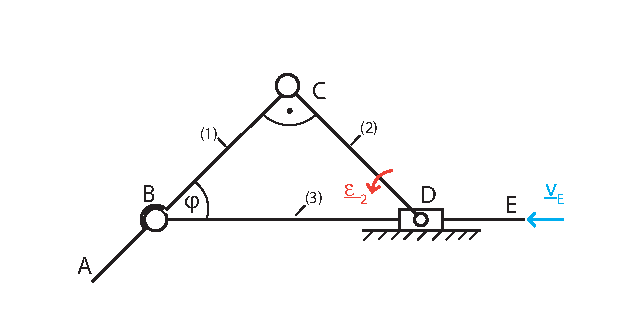
\includegraphics[width=.65\paperwidth]{Képek/2009.10.13_B.pdf}
\end{center}

\vspace{2em}
\underline{\textbf{Feladatok:}}
\begin{enumerate}
    \item Rajzolja be az brába az (1) rúd pillanatnyi sebességpólusát! Határozza meg az A pont
    sebességét!
    \item Adja meg az (1) rúd szöggyorsulását és számitsa ki az E pont pillanatnyi gyorsulását!
    \item Készitsen külön ábrát és jelleghelyesen adja meg az (1) rúd gyorsuláspólusának helyét!
    \item Vizsgálja a (3) rúd B pontjának mozgását a (2) rúdhoz képest! Készitsen külön ábrát és
    jelleghelyesen rajzolja be a B pont szállitó- és relativ sebességét, valamint a B pont Coriolis gyorsulasat!
\end{enumerate}
%------------------------------------------------------------------------------------------
%------------------------------------------------------------------------------------------
%------------------------------------------------------------------------------------------
\newpage

\setstretch{1.6}
\begin{center}
    \textbf{\LARGE{Dinamika}}\\
    1. Zárthelyi\\
    2010.10.11. B csoport
\end{center}
Az ábrán vázolt kétcsuklós robotkar C végpontja a szaggatott vonallal jelzett egyenes pályán mozog. A pályához tartozó befutási törvényt a \(\xi(t)\) függvény adja meg. A robotkart az ábra \(t = 0\) pillanathoz tartozó helyzetben mutatja.\\\\
\underline{\textbf{Adatok:}}\\
$l_1 = 0,3 [m]$\\
$l_2 = 0,2 [m]$\\
$\varphi_1 = 60 [^\circ]$\\
$\varphi_2 = 30 [^\circ]$\\
$\xi(t) = b \cdot t^2 + c \cdot t$\\
$b = -1 \left[\dfrac{m}{s^2}\right]$\\
$c = 1 \left[\dfrac{m}{s}\right]$\\
$\alpha = 45 [^\circ]$
\begin{center}
    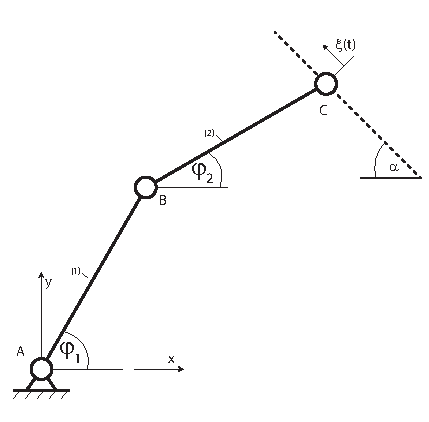
\includegraphics[width=.3\paperwidth]{Képek/2010.10.11.pdf}
\end{center}

\vspace{2em}
\underline{\textbf{Feladatok:}}
\begin{enumerate}
    \item Határozza meg szerkesztéssel a feladatlapon a (2) rúd pillanatnyi sebességpólusának
    helyzetet!
    \item A vázolt helyzetben adja meg az (1) és (2) rudak pillanatnyi sebességállapotát jellemző
    vektorokat a berajzolt \(\{x,y,z; A\}\) koordináta rendszerben!
    \item Számitsa ki a (2) rúd szöggyorsulását és adja meg B pont gyorsulását!
    \item Jelleghelyesen rajzolja be a (2) núd pillanatnyi gyorsuláspólusának helyzetét!
\end{enumerate}
%------------------------------------------------------------------------------------------
%------------------------------------------------------------------------------------------
%------------------------------------------------------------------------------------------
\newpage

\setstretch{1.6}
\begin{center}
    \textbf{\LARGE{Dinamika}}\\
    1. Zárthelyi\\
    2010.10.12. B csoport
\end{center}
Az ábrán vazolt robotkar A és C végpontja az egymástól \(l\) távolságra elhelyezkedő vezetékeken mozog. Az \(l\) hosszúságú (1) és (2) karok közös B pontja a szaggatott vonallal jelzett egyenes pályán mozog. A pályához tartozó befutási törvényt a \(\eta(t)\) függény adja meg. A robotkart az ábra a \( t = 0\) pillanathoz tartozó helyzetben mutatja. D pont az (1) rúd felezőpontja.\\\\
\underline{\textbf{Adatok:}}\\
$l = 1 [m]$\\
$\eta(t) = l - b\cdot e^{-ct}$\\
$b = -1 \left[\dfrac{m}{s^2}\right]$\\
$c = 1 \left[\dfrac{m}{s}\right]$\\
$\alpha = 45 [^\circ]$
\begin{center}
    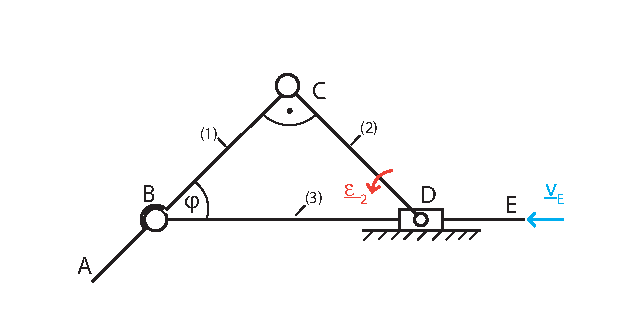
\includegraphics[width=.35\paperwidth]{Képek/2009.10.13_B.pdf}
\end{center}

\vspace{2em}
\underline{\textbf{Feladatok:}}
\begin{enumerate}
    \item Határozza meg szerkesztéssel a feladatlapon az (1) és (2) rudak pillanatnyi
    sebességpólusainak helyzetét!
    \item A vázolt helyzetben adja meg az (1) és (2) rudak pillanatnyi sebességállapotát az A illetve a C ponthoz rendelt kinematikai mennyiségekkel a berajzolt \(\{x,y,z; A\}\) koordináta rendszerben!
    \item Számitsa ki az (1) és (2) rudak szöggyorsulásait és adja meg az A és C pontok
    gyorsulásait!
    \item Számitsa ki és jellephelyesen raizolja be a fenti ábrába a D pont pillanatnyi gyorsulásának tangenciális és normális komponenseit! Határozza meg a D pont pályájának pillanatnyi görbületi sugarát!
\end{enumerate}
%------------------------------------------------------------------------------------------
%------------------------------------------------------------------------------------------
%------------------------------------------------------------------------------------------
\newpage

\setstretch{1.6}
\begin{center}
    \textbf{\LARGE{Dinamika}}\\
    1. Zárthelyi\\
    2011.10.13. 1. csoport
\end{center}
Az ábrán látható forgattyús mechanizmus síkmozgást végez. A mozgás során a bal oldali dugattyú
C pontja ismert sebességgel mozog, pillanatnyi gyorsulása zérus.\\\\
\underline{\textbf{Adatok:}}\\
$v_C = 3 \left[\dfrac{m}{s}\right]$\\
$a_C = 0 \left[\dfrac{m}{s^2}\right]$\\
$r = 0.05 [m]$\\
$l_1 = l_2=l = 0,12 [m]$\\
\begin{center}
    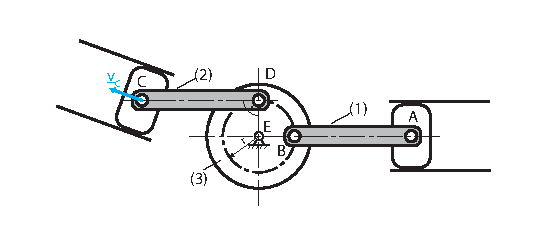
\includegraphics[width=.65\paperwidth]{Képek/2011.10.13.pdf}
\end{center}

\underline{\textbf{Feladatok:}}
\begin{enumerate}
    \item Jelölje be az ábrába az (1) és (2) jelü rudak sebességpólusait \((P1, P2)\)!
    \item Határozza meg az (2) és (3) számú testek szögsebességeit \((\omega_2 =?, \omega_3 =?)\)!
    \item Számitsa ki a (3) jelü test szöggyorsulását \((\varepsilon_3 = ?)\)!
    \item Határozza meg a (3) számú test B pontjának gyorsulását \((a_b =?)\)! Adja meg a
    tangenciális és a normális gyorsulások komponenseit, majd rajzolja be azokat
    jelleghelyesen az ábrába \((\alpha_{Bt} =?, \alpha_{Bn} = ?)\)!
    \item Rajzolja bele az ábrába jelleghelyesen a (2) számú rúd gyorsuláseloszlását a CD szakasz
    mentén!
    \item Az (1) számú rudat mozgó vonatkoztatási rendszernek választva, rajzolja be
    jelleghelyesen az ábrába a baloldali dugatty C pontjának szállitó és relatív sebességét
    \((V_{Cszall} = ?, \beta_c = ?)\)!
\end{enumerate}

%------------------------------------------------------------------------------------------
%------------------------------------------------------------------------------------------
%------------------------------------------------------------------------------------------
\newpage

\setstretch{1.6}
\begin{center}
    \textbf{\LARGE{Dinamika}}\\
    1. Zárthelyi\\
    2015/16 1. csoport
\end{center}
Az ábrán látható forgattyús mechanizmus síkmozgást végez. A (2) jelű, tisztán gördülő korong a vizsgált pillanatban az R sugarú kényszerpálya legalsó pontjában van. Az (1) vízszintes rúd B végpontja csuklóval kapcsolódik a koronghoz, A végpontja pedig egy vízszintesen elmozdulni képes csuszkával van csuklós kapcsolatban. A korong szögsebessége és szöggyorsulása adott. Az irányok az ábrának megfelelőek. Minden eredményt a megadott koordináta rendszerben adjon meg.\\\\
\underline{\textbf{Adatok:}}\\
$\omega_2 = 3 \left[\dfrac{rad}{s}\right]$\\
$\varepsilon_2 = 10 \left[\dfrac{rad}{s^2}\right]$\\
$R = 2 [m]$\\
$r = 0,5 [m]$\\
$l = 1 [m]$\\
\begin{center}
    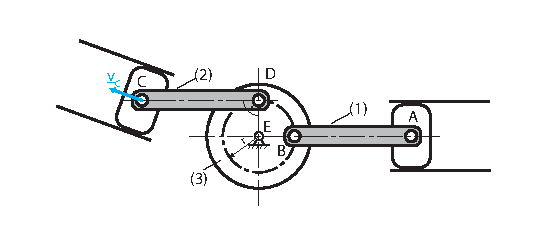
\includegraphics[width=.35\paperwidth]{Képek/2011.10.13.pdf}
\end{center}

\underline{\textbf{Feladatok:}}
\begin{enumerate}
    \item Jelölje be az ábrán a B pont sebességének irányát és a (1) jelú rúd sebesség pólusát \(P_1\)!
    \item Határozza meg a B pont sebességét és az (1) rúd szögsebességét! Az A pont sebességét és C pont sebességét!
    \item Határozza meg a C pont gyorsulását!
    \item Számítsa ki a B pont gyorsulását és az adott (1) test szöggyorsulását! határozza meg a korong gyorsuláspólusának helyét!
\end{enumerate}
\end{document}